%----------------------------------------------------------------------------
\chapter{Object detection}

Computer vision is a scientific field that deals with how computers extract high-level information from digital images or videos. The input can be various (like a three-dimensional point cloud), but for the sake of simplicity, I assume they are two-dimensional images. In general, computer vision tries to automate tasks that the human visual system can do, and there are numerous ones:

\begin{itemize}
  \item The easiest is \textit{image classification}, where the input is an image, and the output is a simple class. But if the image contains multiple classes at the same time, we cannot find them with this approach.
  \item \textit{Semantic segmentation} is a task where each input image pixel is classified, and the output is a mask containing pixel-level class predictions. But if there are multiple instances of the same class in the image, we cannot distinguish them.
  \item The solution to this problem can be \textit{object segmentation}, where each object gets a different Id in the output mask, even if they are from the same class. This task is a more advanced pixel-level classification, but it usually constraints the maximum amount of objects of the same type per image.
  \item Another approach to distinguish multiple instances of the same type can be \textit{object localization}, where a bounding box is drawn around an object in the image. This can be solved as a regression problem. But if we are interested in the object's location and type at the same time, it is not enough.
  \item This is where multi-box \textit{object detection} comes into play, unifying the localization (regression) and classification problem. The outputs are bounding boxes having properties \(X\textsubscript{min}, Y\textsubscript{min}, X\textsubscript{max}, Y\textsubscript{max}\), and the \(class\). The location information can be encoded in numerous ways, like \((X\textsubscript{min}, Y\textsubscript{min}, width, height)\) or \((X\textsubscript{center}, Y\textsubscript{center}, \frac{width}{2}, \frac{height}{2})\). There are approaches where bounding boxes have extra attributes like rotation angle or further coordinates for 3D object detection. In the following, I discuss 2D bounding box detection without rotation.
\end{itemize}

Object detection is a difficult task to algorithmize, so it is worth turning to the toolkit of neural networks. Although there are classical machine learning solutions, like HOG linear SVM-based detectors\cite{VehicleDetectionHOG-SVM}, deep learning-based object detection has been a research hotspot in recent years due to its powerful learning ability\cite{ObjDetDeepLearningReview}.

In the following part, I discuss the main concepts and explain different metrics and model evaluation protocols. Then building on this knowledge, I present numerous detector architectures and their novel ideas in chronological order.

\section{Intersection over Union}

The first essential operation to understand is \textit{Intersection over Union}. It is calculated as follows: 

\[IoU=\frac{area\textsubscript{overlap}}{area\textsubscript{union}}\]

It measures how much a box overlaps with another box. This simple operation is used extensively in object detection, matching ground truth boxes with anchor boxes (at training). It is also used in non-maximum suppression\cite{NMS} for removing multiple predictions of the same object (at inference). Recently, it is also used as a differentiable localization loss function (CIoU\cite{IoULosses}) between ground truth boxes and predicted boxes (at training). Sometimes, there are predefined IoU thresholds for the different usages. For example, above 0.5, an anchor box is interpreted as positive w.r.t. a ground truth box, but below as a negative sample. These are hyperparameters to tune.

\begin{figure}[htb]
 \centerline{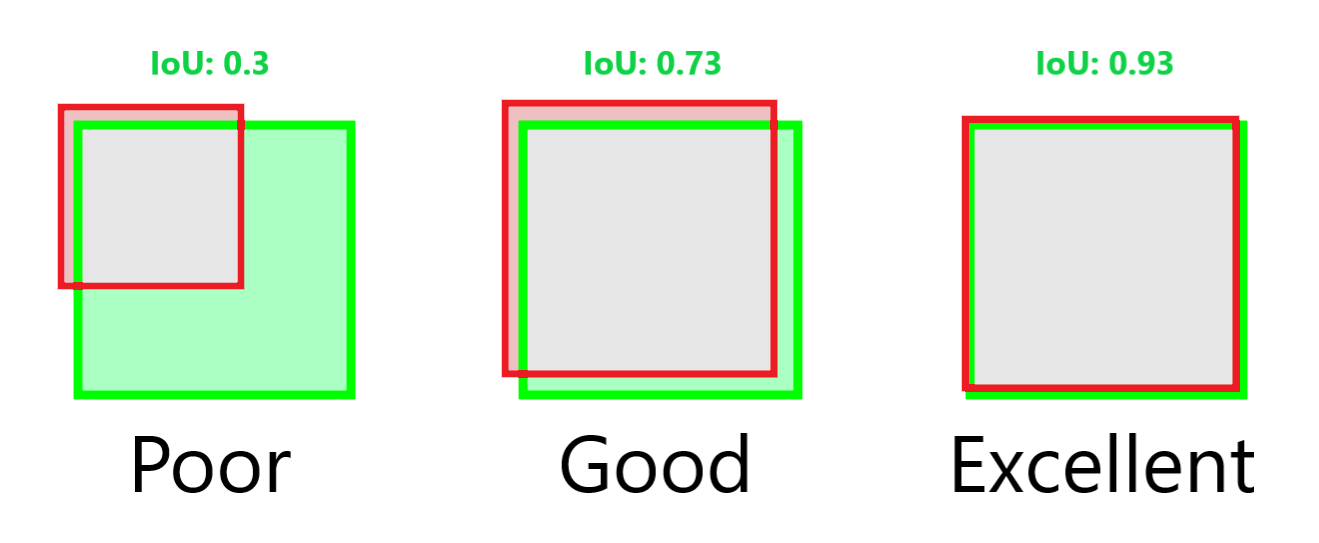
\includegraphics[width=1.0\columnwidth]{.//Figure/Detector/IoU.png}}
 \caption{Intersection over Union of different bounding boxes.}
 \label{fig:IoU}
\end{figure}

\section{Anchor boxes}

The anchor box examples and explanation points are partly inspired by the following article\cite{AnchorBoxes}. When an image is passed through an object detector, it makes box predictions in the order of thousands, of which only a few are real objects. The following example illustrates and explains why detectors work like this.

\subsection{The problem}

\begin{figure}[htb]
 \centerline{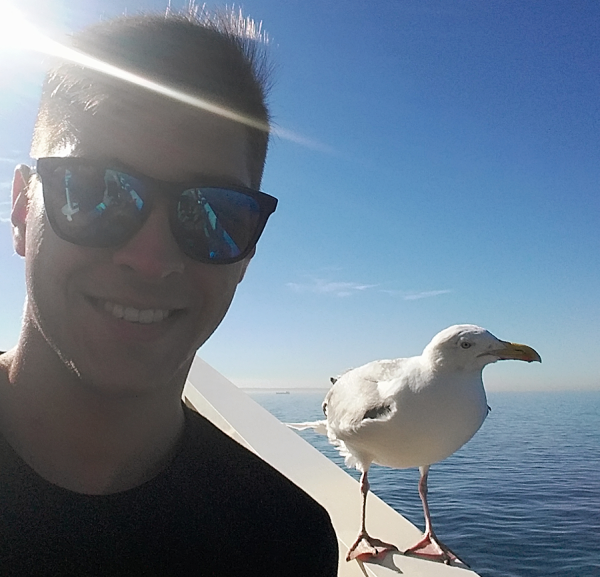
\includegraphics[width=0.5\columnwidth]{.//Figure/Detector/human_bird.png}}
 \caption{An example image with different objects.}
 \label{fig:human_bird}
\end{figure}

Suppose there is a model which can detect two objects in an image. This model gets the input image on Figure \ref{fig:human_bird}. While training, the model needs to know which predictions are correct to be able to learn. But there can be multiple right solutions:

\begin{itemize}
  \item \textit{predictor 1}: human, \textit{predictor 2}: bird
  \item \textit{predictor 1}: bird, \textit{predictor 2}: human
\end{itemize}

When the detector outputs the following:

\begin{itemize}
  \item \textit{predictor 1}: bird, \textit{predictor 2}: bird
\end{itemize}

It is unclear which predictor is correct and which is not. The network needs to know which of its two predictors is responsible for detecting the human or the bird. For this, predictors can specialize in specific things (object size, aspect ratio, objects in different parts of the image). Modern object detectors use all of these specializations with their predictors. In this example, the optimal task sharing is that \textit{predictor 1} is responsible for objects on the left while \textit{predictor 2} is for objects on the right. This way, the correct model output is clear:

\begin{itemize}
  \item \textit{predictor 1}: human, \textit{predictor 2}: bird
\end{itemize}

\subsection{Anchor-based operation}

Anchor-based object detectors do the same on a bigger scale the following way.

\begin{itemize}
  \item They generate thousands of predefined anchor boxes; each mapped to a single predictor. One predictor is responsible for finding objects of its anchor box's location, size, and aspect ratio.
  \item When training, IoU is calculated for each ground truth box and anchor box. Anchor box with the highest IoU w.r.t. the ground truth is responsible for detecting that ground truth box.
  \item If the calculated highest IoU is above an upper threshold (say 0.5), the corresponding anchor box needs to detect the object. If the highest IoU is below a lower threshold (say 0.3), the anchor box must predict no object. If none is met, the ground truth has too low maximum IoU to be positive but too high to be negative. In this case, the anchor box is ambiguous, so not used in the current loss calculation.
  \item The predictor of the anchor box outputs the offsets/rescale ratios. In some detector architectures, like YOLO, a predictor is only responsible for a ground truth box if the box's center is in the predictor's grid cell.
\end{itemize}

This anchor-based approach is used in many detector solutions and works quite well.

\subsection{Limitations}

The number of anchor boxes is in the order of thousands. Some architectures like RetinaNet\cite{RetinaNet} have more than 100,000 anchor boxes in specific cases. Calculating IoU and then predicting boxes in this order of magnitude is resource-intensive and a potential bottleneck.

The massive number of anchor boxes means a positive-negative class imbalance because there are way more anchor boxes than ground truth boxes. Most of the anchor boxes are assigned as negatives and just a tiny portion of them as positives. Many negative samples suppress the gradients of the positive ones, and the model potentially does not learn. There are various techniques to solve this problem, like hard negative mining\cite{SSD} (SSD), objectness score-based loss value reduction\cite{YOLO} (YOLO), or a dynamically scaling focal loss function\cite{RetinaNet} (RetinaNet). I describe each of these solutions in the discussion of the specific architectures.

The last problem is that anchor boxes are parameter-sensitive. Datasets have boxes of different sizes and shapes, and if the predefined anchors do not fit the properties of the ground truth boxes, low IoU values are calculated. Thus, the network does not even know that ground truth objects exist and cannot predict them. There are different approaches to finding ideal anchor configurations. Hand-crafted bounding boxes are used in SSD, while YOLOv3\cite{YOLOv3} uses a k-means algorithm to estimate ideal values w.r.t. a given dataset.

To illustrate the phenomenon, Figure \ref{fig:anchor_bad_match} shows 1\% of the default anchor boxes (for the MS-COCO dataset) of RetinaNet. The matched bounding boxes are the following when training and evaluating the same model on the WiderFace dataset. Only a few ground truth boxes overlap with any of the anchor boxes. Thus the majority of the faces cannot be detected.

\begin{figure}[htb]
 \centerline{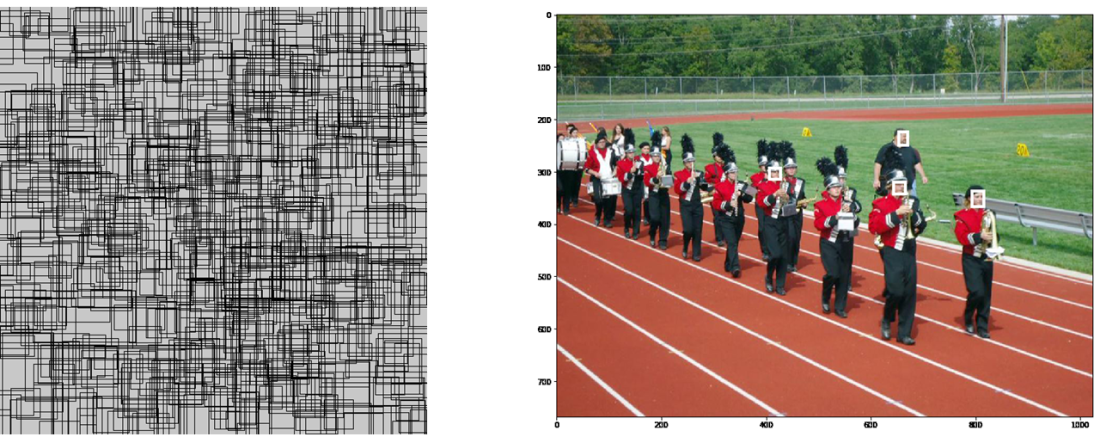
\includegraphics[width=1.0\columnwidth]{.//Figure/Detector/anchor_bad_match.png}}
 \caption{Left: 1\% of the default RetinaNet anchor boxes. Right: The detector can find only a few faces with this configuration. Source: \cite{AnchorBoxes}}
 \label{fig:anchor_bad_match}
\end{figure}

Figure \ref{fig:anchor_good_match} shows 1\% of the adjusted anchor boxes, where the size of the smallest anchors has been reduced. With this configuration, all face ground truth boxes have been matched by at least one anchor box, so the model can detect them.

\begin{figure}[htb]
 \centerline{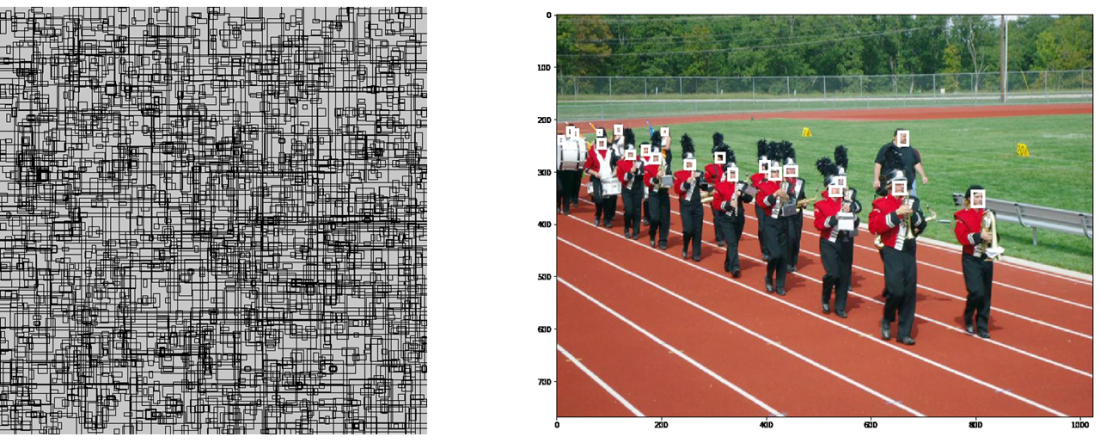
\includegraphics[width=1.0\columnwidth]{.//Figure/Detector/anchor_good_match.png}}
 \caption{Left: 1\% of the adjusted (smaller) anchor boxes. Right: With the proper anchors, the detector can localize all of the faces. Source: \cite{AnchorBoxes}}
 \label{fig:anchor_good_match}
\end{figure}

Finally, it is also important to note that the IoU value depends on the center of the compared boxes. Even if we use correctly small anchor boxes, if the strides between them are too high, some ground truth boxes can be missed. The upper IoU threshold can be lowered to address this issue, or adding a denser anchor grid-level also helps (increasing the number of anchors and thus is more resource-intensive).

\section{Non-maximum suppression}

When there is a specific object in an image, the cell in the grid responsible for finding it outputs high probability predictions. Usually, the adjacent cells also output pretty good proposals for the same object. But we only need one bounding box for one object. The others need to be suppressed. The algorithm to find the best match and discard the others is called non-maximum suppression\cite{NMS} (NMS). Its steps are the following:

\begin{itemize}
  \item The method first selects a proposal box with the highest confidence score, removing it from the initial box list \textit{B} and adding it to output boxes list \textit{P}.
  \item Next, for all the other boxes in \textit{B}, IoU is calculated w.r.t. the box in \textit{P}. Each box with an IoU value above a threshold is discarded from \textit{B}.
  \item This simple algorithm is repeated until \textit{B} gets empty. When this happens, \textit{P} contains the final list of the predicted boxes.
\end{itemize}

\begin{figure}[H]
 \centerline{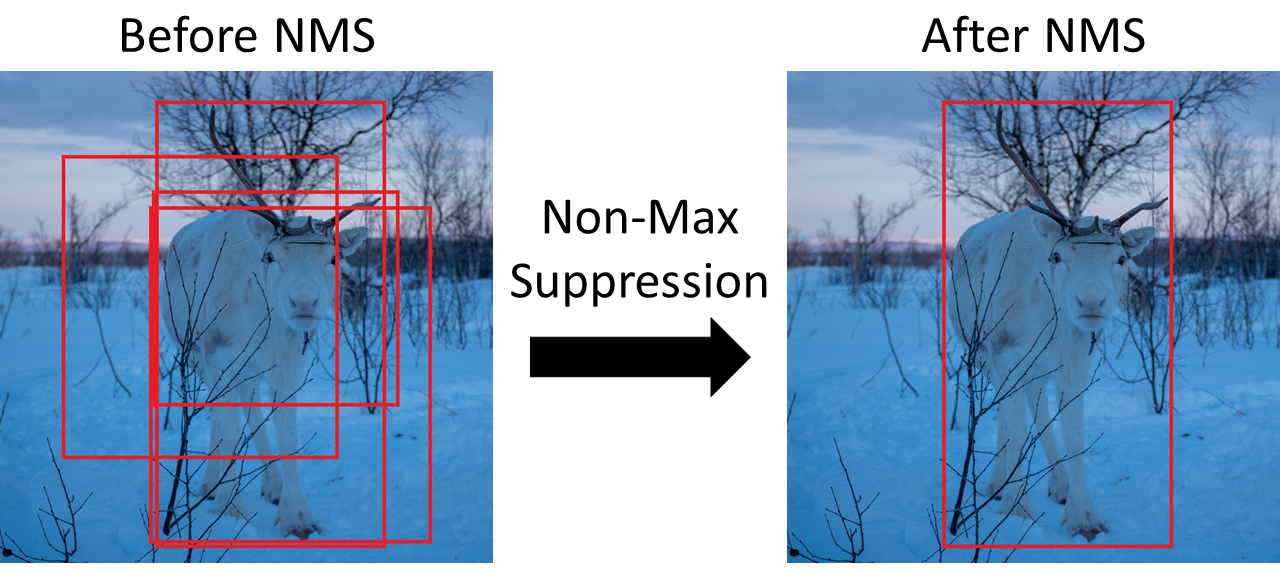
\includegraphics[width=1.0\columnwidth]{.//Figure/Detector/NMS.png}}
 \caption{The effect of the non-maximum suppression algorithm.}
 \label{fig:NMS}
\end{figure}

This algorithm has numerous variants, like Combined NMS, where the IoUs are calculated between boxes classified as the same class. This avoids suppressing boxes of different objects close to each other.

\section{Loss function}

Object detection unifies a localization (regression) and a classification problem. These are tasks with different properties: one is in a continuous domain, while the other is in a discrete. In early two-stage detectors like R-CNN\cite{R-CNN}, the localization and classification tasks are entirely separated. Each module could be trained with the appropriate loss function individually. When training detector systems in an end-to-end manner, we need to optimize both at the same time. For this, object detection usually has a composite loss function, incorporating penalties for both things. The single output value of the cost function is the error, which is backpropagated through the network to optimize the model: calculate the gradients and update weights. This is why a suitable loss function is crucial to train an object detector.

When training in an end to end manner, the cost function incorporates both task penalties. It is important to weigh the classification and localization errors to avoid any of them dominating the error. There are usually hyperparameters to weigh those loss components.

Over time, many loss functions emerged. The original YOLO\cite{YOLO} uses sum-squared error for both problems, which can work by introducing a third simple loss component (objectness score), but has its limitations. SSD\cite{SSD} uses Softmax for classification and Smooth L1 for localization. It adds an extra empty class and hard negative mining to balance class inequality, different from YOLO. RetinaNet\cite{RetinaNet} introduced focal loss for classification, a function handling class inequality by downscaling easy examples. YOLOX\cite{YOLOX} uses a differentiable IoU function\cite{NMS} (Complete IoU) for calculating localization loss. There are many different approaches with their pros and cons. I discuss them more thoroughly in the detector architectures section.

\section{Metrics}

Choosing the right metrics is crucial to train and evaluate a detector appropriately for the task. If we solely concentrate on the single loss value, we easily miss out on details like how well the model localizes (where is the object?) or how well it classifies (is it a vehicle?). They may suggest different things about the network. For example, in a single-stage architecture (discussed later), classification depends primarily on the backbone, while detection is mainly the task of the last convolutional layers. Thus, if the classification performance is weak, we may modify the backbone to improve it.

Some metrics appear for most protocols, which I briefly describe here partly based on \cite{mAP}. The following concepts assume a binary decision problem, but this can be extended to a multi-class decision by saying positive if the target class is predicted or negative in any other case. I use the following abbreviations: \(T\textsubscript{p}\): true positive, \(T\textsubscript{n}\): true negative, \(F\textsubscript{p}\): false positive, \(F\textsubscript{n}\): false negative.

\textit{Acccuracy} is the ratio of trues among all predictions. We can calculate it as follows:

\[Accuracy=\frac{T\textsubscript{p}+T\textsubscript{n}}{Total}\]

\textit{Precision} gives the ratio of ground truth positives among all positive predictions.

\[Precision=\frac{T\textsubscript{p}}{T\textsubscript{p}+F\textsubscript{p}}\]

The \textit{Recall} metric is the true positive hit ratio among all ground truth positives.

\[Recall=\frac{T\textsubscript{p}}{T\textsubscript{p}+F\textsubscript{n}}\]

\textit{Average Precision} is the area under the precision-recall curve.

\[AP=\int_{0}^{1} p(r)\,dr \]

The following example demonstrates how to calculate Average Precision. Table \ref{tab:sample_detection} shows the result of some evaluations:

\begin{table}[htb]
\caption{Sample detection results in a tabular form.}
\label{tab:sample_detection}
\noindent
\centering
\begin{tabular*}
{\columnwidth}{@{\extracolsep{\stretch{1}}}*{4}{r}@{}}
    Id & Correct (IoU>0.5)? & Precision & Recall\\ \hline
    $1$ & $True$ & $1.00$ & $0.33$ \\
    $2$ & $True$ & $1.00$ & $0.66$ \\
    $3$ & $False$ & $0.67$ & $0.66$ \\
    $4$ & $True$ & $0.75$ & $1.00$ \\
    $5$ & $False$ & $0.60$ & $1.00$ \\          
\end{tabular*}
\end{table}

The calculation of detection 4 of Table \ref{tab:sample_detection} is the following: Precision is the proportion of  \(T\textsubscript{p}\)s so far \(\frac{3}{4}=0.75\), Recall is the proportion of  \(T\textsubscript{p}\)s out of the possible positives \(\frac{1}{3}=1\). Recall continually increases as we go down on the prediction ranking. However, precision can follow a zig-zag pattern (decreases with  \(F\textsubscript{p}\)s and increases with \(T\textsubscript{p}\)s). Average precision is the area under the precision-recall curve. The AP of the current example is on Figure \ref{fig:precision_recall}. As precision and recall values are always between 0 and 1, AP falls within this boundary, too.

\begin{figure}[htb]
 \centerline{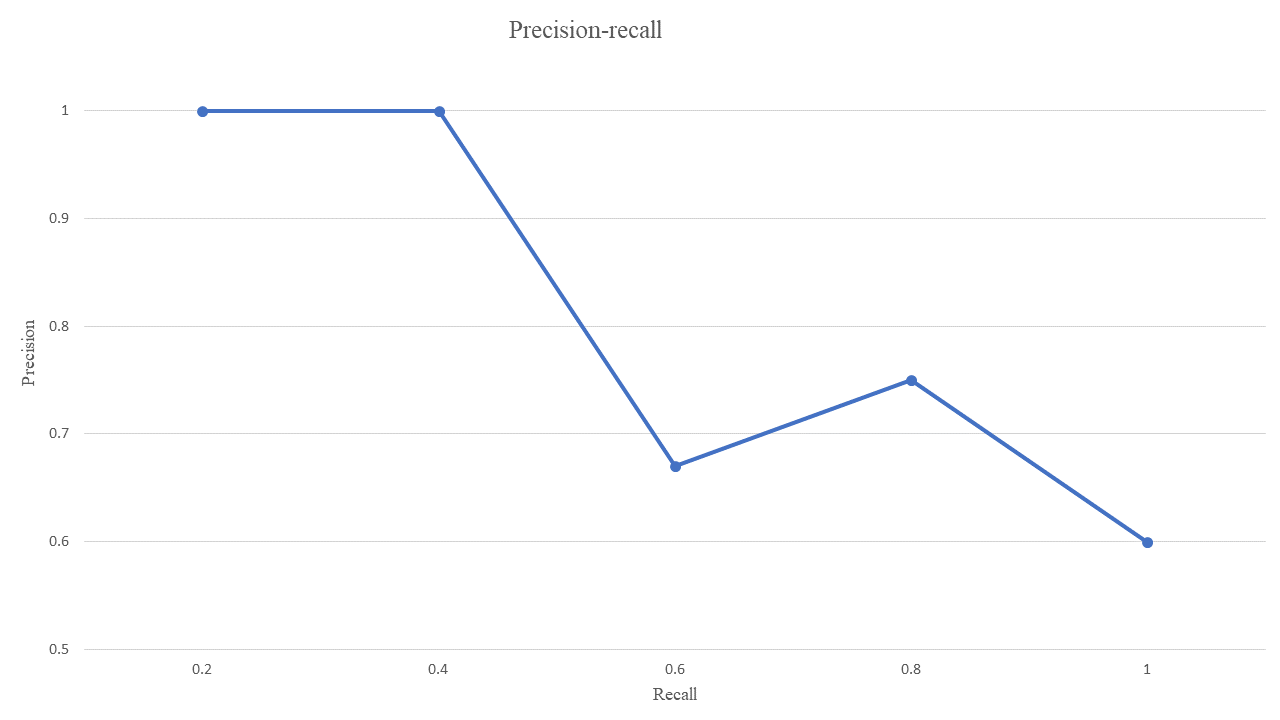
\includegraphics[width=0.8\columnwidth]{.//Figure/Detector/precision_recall.png}}
 \caption{Sample detection AP in a line chart.}
 \label{fig:precision_recall}
\end{figure}

\textit{Interpolated Average Precision} divides the recall value from 0 to 1 into n points. It is used to smooth out the zig-zag pattern of AP (at each recall level, replacing each precision value with the highest precision found to the right of that recall level\cite{IntroInfoRetrieval}). The IAP of the example is on Figure \ref{fig:transformed_precision_recall}. Interpolated AP is calculated based on the area below the smoothed values. It is the basic idea behind the mAP metric variants.

\[IAP=\frac{1}{n}\sum_{n\in(0.0 ... 1.0)} AP\textsubscript{n}\]

\begin{figure}[htb]
 \centerline{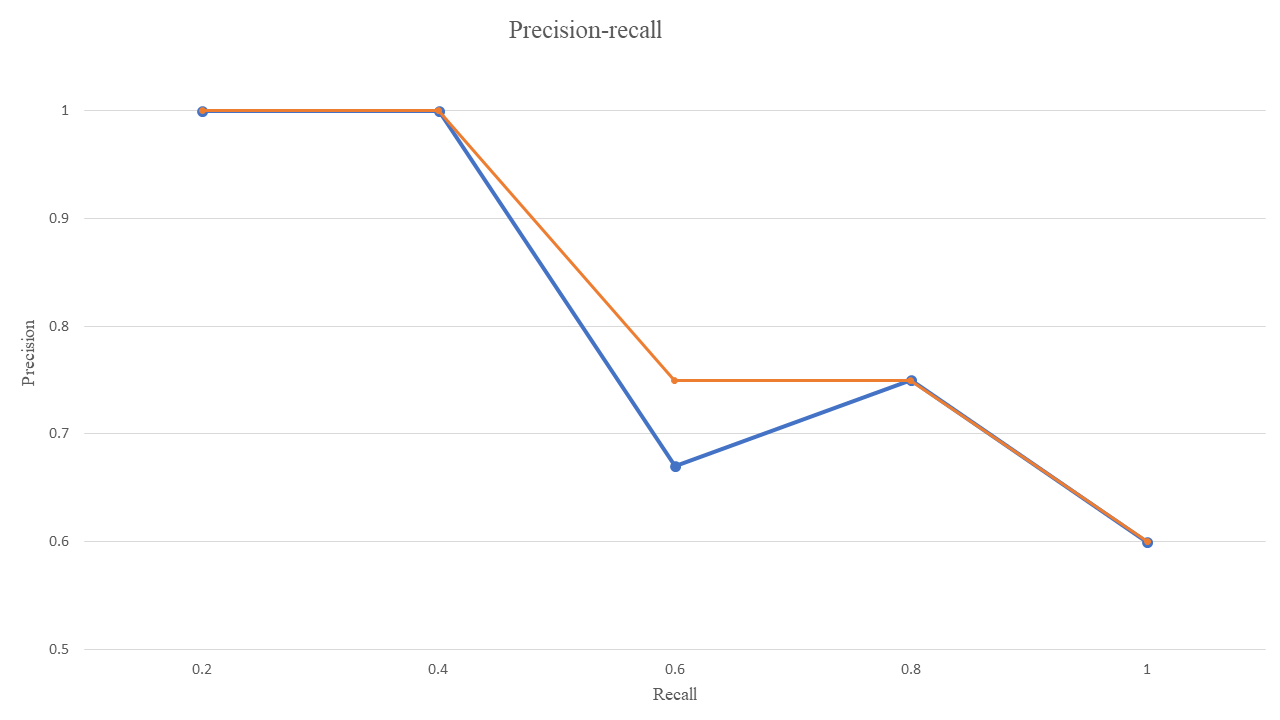
\includegraphics[width=0.8\columnwidth]{.//Figure/Detector/transformed_precision_recall.png}}
 \caption{Metric comparison on the previous sample: \textcolor{blue}{AP}, \textcolor{orange}{IAP}.}
 \label{fig:transformed_precision_recall}
\end{figure}

The last metric discussed here is \textit{mean Average Precision (mAP)}. There are numerous types of mAP. In COCO, a 101-point interpolated AP is used, which is the average over 10 IoU levels starting from 0.5 to 0.95 with a step size of 0.05. Hereafter, I refer to the COCO implementation by this name.

\section{Protocols}

There is no consensus about the evaluation metrics of the object detection problem. Different competitions such as PASCAL VOC\cite{PascalVOC}, MS-COCO\cite{MS-COCO}, or Google Open Images Challenge\cite{OID} have their ways to measure performance\cite{mAP}.

PASCAL VOC\cite{PascalVOC} has introduced mAP to evaluate detectors' quality with an 11-point interpolated AP definition.

COCO detection metrics\cite{MS-COCO} are similar but have additional measures such as mAP at different IoU thresholds from 0.5 to 0.95. There are also precision/recall statistics for small \((area < 32^2)\), medium \((32^2 \leq area < 96^2)\), and large \((area \geq 96^2)\) objects.

Open Images V2 detection metrics\cite{OID} focus on average precision for each class and among all classes, but there are no metrics for objects grouped by their size. OID classes are organized in a hierarchy (e.g., car groups several specific classes like limousine or van). If a model claims that a van is a car, it is not punished as drastically as if it had claimed it was a cat.

\section{CNN architectures}

Before we deep-dive into the detector architectures, I discuss some of the most popular CNN versions popular in object detectors.

Convolutional Neural Network (CNN) models are widely used in deep learning. They usually stack multiple convolutional layers with nonlinearity (usually ReLU) and pooling layers. Because of pooling, the input feature spatially gets smaller, but by convolution, the dimensionality increases. Object detection architectures usually use CNNs as feature extractor backbones. Other approaches, like transformer-based detectors, exist, but current real-time systems use CNNs. Therefore, I present some of the most popular variants used in object detection.

Early convolutional networks were primarily engineered for image classification problems. The first stepping stone I mention is LeNet-5\cite{LeNet} from 1998, created by Yann LeCun for classifying hand-written digits. The next one is AlexNet\cite{AlexNet}, which won the 2012 ImageNet ILSVRC classification challenge\cite{ILSVRC}; this model stacked multiple convolutional layers on top of each other without pooling and is a much deeper network. GoogLeNet\cite{GoogLeNet} won the ILSVRC challenge in 2014; the novel idea of this network was the inception module, where each block contains multiple different convolutional operations to extract features of more diverse patterns. These models are not usually used for object detection, but the ideas they introduce have been extensively used.

VGG-16\cite{VGG16} was the first popular CNN used in object detectors. In 2014, it was the runner-up behind GoogLeNet in the ILSVRC challenge. This model has a simple structure with 2-3 convolutional layers between each pooling layer (16 layers in total). VGG-16 became a popular detector backbone due to its power and simplicity and the fact that the first detector architectures (Fast R-CNN, SSD) emerged around that time.

ResNet\cite{ResNet} won the ImageNet 2015 challenge. It has introduced skip connections with residual units. Skip connections are helpful because while training, the input signal can make its way across the network, so even if deeper layers have not started learning (their output is close to zero), the network can progress. These residual units help resolve the vanishing gradient problem, making it possible to create deeper trainable networks (around 50-100 layers).

MobileNets are special models optimized for mobile/IoT inference. They are small and fast, but their accuracy is relatively high. Version 2 uses linear bottlenecks and inverted residuals. According to the MobileNetV2 paper\cite{MobileNetV2}, bottlenecks store all the necessary information, and between them, expansion layers serve for extraction with nonlinearities. Thus, bottlenecks are linear layers to prevent nonlinearities from destroying the original information. The other novel idea is that as bottlenecks store the information, shortcuts are only needed directly between them.

There are other popular CNNs used in object detection, like DarkNet, CornerNet, or EfficientNet. Since these are models optimized for detection, I discuss them in the description of the detector architecture associated with them.

\section{Detector architectures}

Generally, there are two types of deep learning-based detector architectures: two-stage (e.g., R-CNN) and one-stage variants (like YOLO, SSD, RetinaNet, CenterNet). I briefly describe the two-stage versions, then more comprehensively the one-stage detectors because they are faster, thus, more suitable for smartphone inference.

\subsection{Two-stage detectors}

Two-stage detectors have this name because first, they propose object candidate regions, then classify these regions. Those steps are executed with different algorithms separately. Until the mid-2010s, complex ensemble machines were the best performing models in object detection.

\subsubsection{Region-based Convolutional Neural Network}

In 2014, Region-based Convolutional Neural Network\cite{R-CNN} (R-CNN) was introduced for detection and segmentation tasks. Its main idea was to use a region proposal for generating category-independent object candidates, then feeding them to a feature extractor CNN. In this arrangement, there is a third module, which is a set of class-specific linear SVMs. In this architecture, the separate modules must be trained independently.

\subsubsection{Fast R-CNN}

In 2015, Fast R-CNN\cite{FastR-CNN} was introduced. It used VGG-16 as a feature extractor and made it possible to train the whole system at once. The main architectural difference to the previous version is that it feeds an input image directly to the CNN to generate a convolutional feature map. Proposals are identified by an RoI (Region of Interest, max-pooling) layer, fed to dense layers outputting coordinates. There is also a softmax layer from the RoI feature vector, which predicts the class of the proposed region. Fast R-CNN is considerably quicker than its predecessor because, for 100 region proposals, there is no need to feed all of them independently to the CNN - RoIs from the same image share computation and memory.

\subsubsection{Faster R-CNN}

The Faster R-CNN\cite{FasterR-CNN} variant from 2016 consists of a fully convolutional RPN (Region Proposal Network) and a Fast R-CNN detector using the output of the former. The RPN is a fully convolutional module predicting offsets for hand-picked prior bounding boxes (anchor boxes). The two networks might share a common set of convolutional layers. RPN is a small network working in a sliding-window fashion, which predicts the regions unlike R-CNN or Fast R-CNN, where a significantly slower selective search algorithm is used for this purpose.

\subsubsection{Mask R-CNN}

The next variant of the R-CNN family is the Mask R-CNN\cite{MaskR-CNN}. It extends Faster R-CNN by adding a small fully-connected network as a third output branch predicting object masks (parallel with localization and classification). In addition, this variant introduces the RoIAlign layer, which accurately maps a region of interest to a smaller feature map without rounding up to integers. This architecture is suitable for both detection and segmentation.

\begin{figure}[htb]
 \centerline{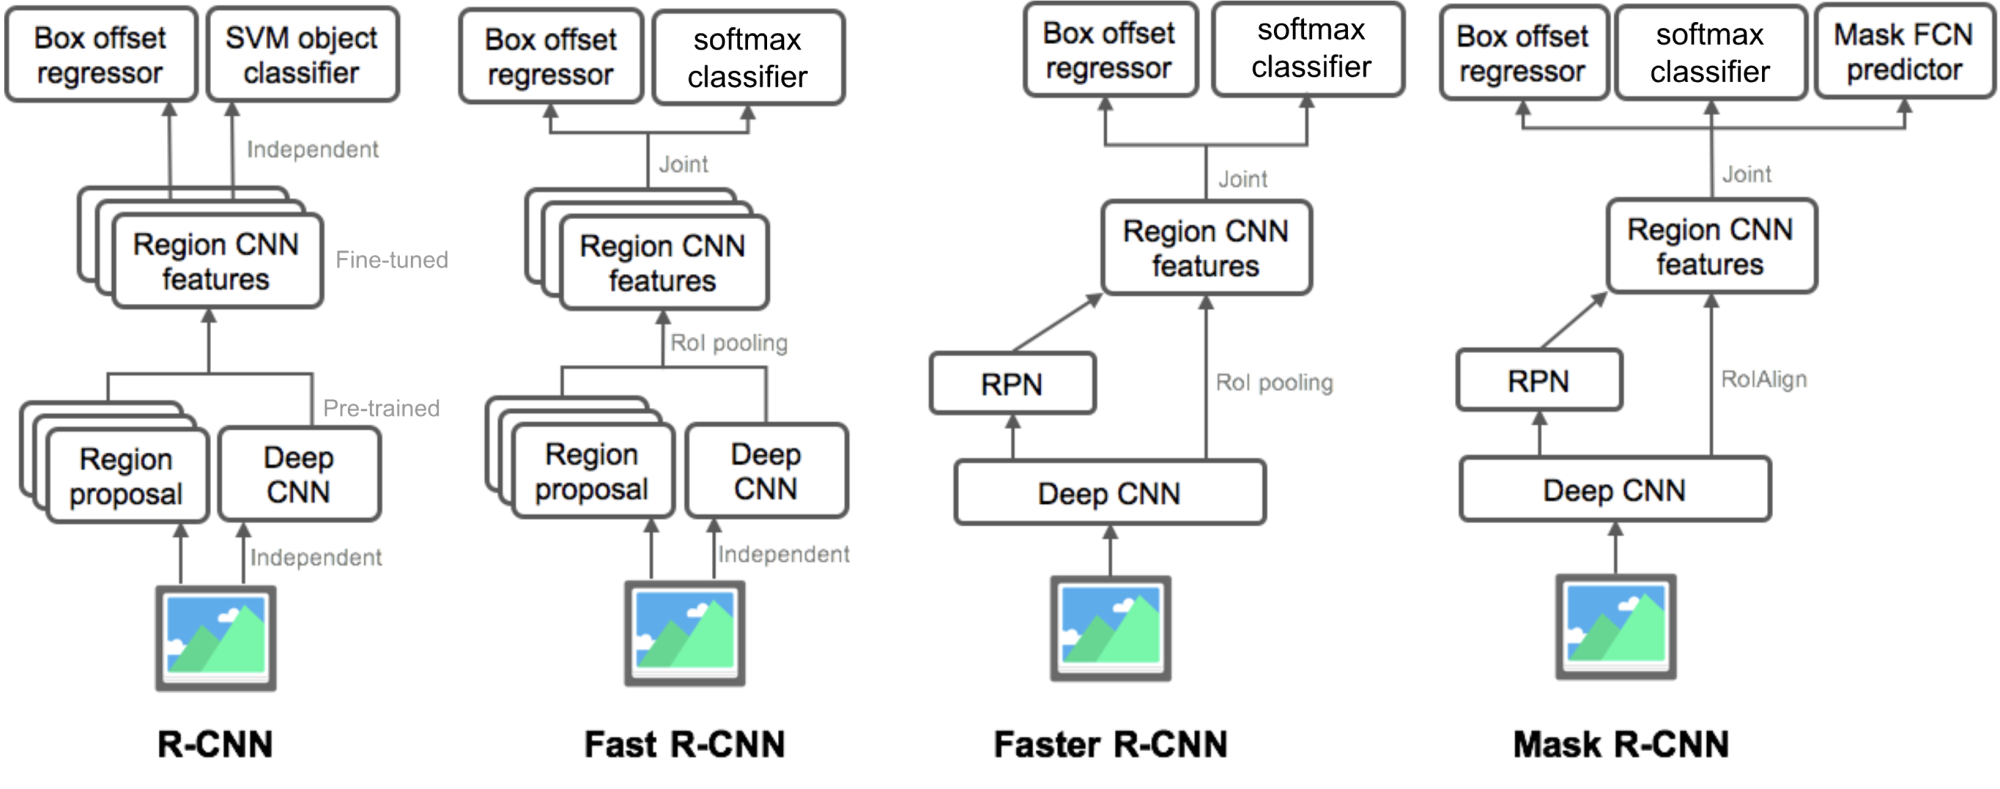
\includegraphics[width=1.0\columnwidth]{.//Figure/Detector/RCNN_family.png}}
 \caption{R-CNN family variants. Source: \cite{ObjDetArchitectures3}}
 \label{fig:RCNN_family}
\end{figure}

Further two-stage detectors, like Libra R-CNN\cite{LibraR-CNN}, apply balanced IoU sampling, FPN, and L1 loss to address the class imbalance problem during training. Powerful anchor-free variants also exist, like RepPoints. However, I do not discuss these particular approaches, as my main goal is to present the basic ideas behind two-staged detectors.

\subsection{One-stage detectors}

Two-stage detectors can achieve high accuracy, but they are usually too slow for real-time application. One-stage detectors are not region-based algorithms; they merge the localization and classification tasks into one network - running detection directly over a dense sampling of possible locations. One-stage detectors are fast by design, but they are usually less accurate.

\subsubsection{You Only Look Once}

The first one-stage detector aiming for real-time inference was You Only Look Once\cite{YOLO} (YOLO). It was introduced in June 2015, initially written in the DarkNet framework. YOLO is a unified architecture with a single network containing 24 convolutional layers and two fully connected ones. The convolutional layers extract features from images, while the dense layers predict coordinates and probabilities. The input image is divided into an \(N \times N\) grid in which a cell is responsible for predicting boxes in its area. In YOLO, one box has six properties: \(X\textsubscript{center}, Y\textsubscript{center}, \frac{width}{2}, \frac{height}{2}, objectness\) and multi-hot encoded \textit{class confidence}. The localization values \((X\textsubscript{center}, Y\textsubscript{center}, \frac{width}{2}, \frac{height}{2})\) are normalized and directly predicted using fully connected layers. A single cell outputs two boxes and their confidence values for every \textit{C} classes, so the total output shape is \(N \times N \times ((2 \times 5)+C)\). This means that one grid cell can detect maximum one object. In YOLO, the loss function is a sum-squared error for both classification and localization. This loss function has the following limitations:

\begin{itemize}
  \item It weights regression (localization) and classification errors the same way, which is not optimal.
  \item The high number of negative samples (in every image, many grid cells do not contain any object) tends to overpower the positive ones, pushing the confidence scores towards zero. This is handled in YOLO by predicting the objectness score and down-scaling bounding box losses with low objectness values.
  \item The loss function equally weights errors in small- and large boxes, but the loss should reflect that slight deviation in large boxes matters less than in small boxes. To address this, YOLO predicts the square root of the bounding box width and height.
\end{itemize}

These problems regarding the loss function have been addressed in later architectures. When it was introduced, YOLO was considered fast and straightforward compared to the state-of-the-art and less likely to predict false positives on the background than two-staged detectors. On the other hand, it makes more localization mistakes (partly related to the loss function) and struggles with small objects.

\begin{figure}[htb]
 \centerline{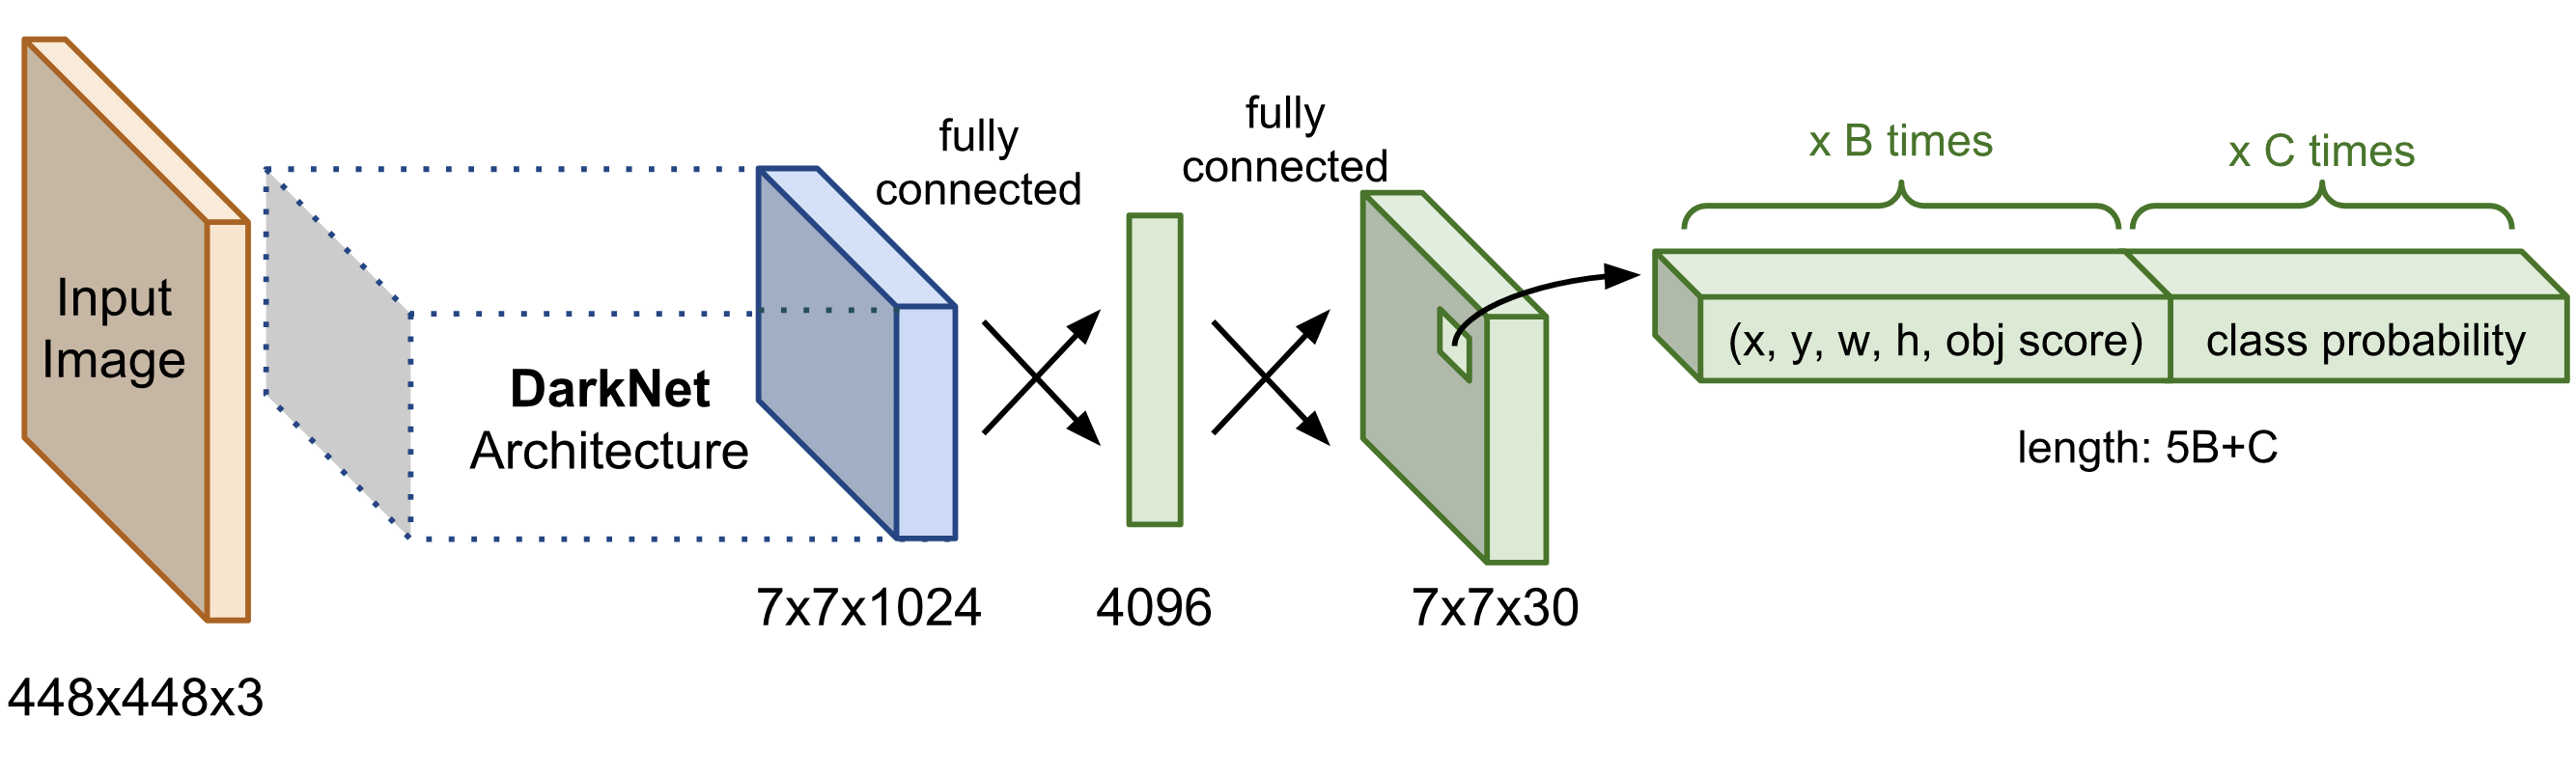
\includegraphics[width=1.0\columnwidth]{.//Figure/Detector/YOLO.png}}
 \caption{The YOLO architecture. Source: \cite{ObjDetArchitectures4}}
 \label{fig:YOLO}
\end{figure}

\newpage
\subsubsection{Single Shot MultiBox Detector}

Single Shot MultiBox Detector\cite{SSD} (SSD) was introduced in December 2015. In the first part of this architecture, a general-purpose image classification CNN (VGG-16) is used as the backbone. After that, multiple convolutional layers implement a pyramidal structure for multi-scale object localization as shown in Figure \ref{fig:SSD}. These layers progressively decrease in size towards the end of the architecture, allowing detections at various scales (unlike YOLO, which operates on a single-scale feature map). This makes it possible to detect objects of different sizes better at the cost of more resource intensity.

SSD uses a set of default bounding boxes for each cell on each feature map. For training, anchor boxes of different sizes and IoU calculations are needed. This is a fundamentally different approach than YOLO. The box properties are \(X\textsubscript{center}, Y\textsubscript{center}, \ln{\frac{width}{2}}, \ln{\frac{height}{2}}\), and \(confidence\), where the first four values are offsets and resizing ratios of the corresponding anchor box. The predictor outputs the logarithm of the vertical- and horizontal rescaling factors, which is an easier representation for neural networks and thus speeds up training. Unlike YOLO, SSD has no objectness score prediction and loss downscaling, but encodes non-objects as an empty class. The loss function is the sum of the classification loss (softmax over the class confidences) and the localization loss (Smooth L1; a quadratic function below a threshold and an absolute function above). SSD has numerous anchor boxes in multiple scales, and the majority of them do not contain any object for a single image. There is no objectness score-based loss downscaling, so the positive-negative class imbalance is a significant problem. As a remedy, hard negative mining is applied after each matching step, selecting the top negative samples with the highest losses so that the positive-negative sample ratio is 1:3. The other negatives are discarded, leading to faster and more stable training.

\begin{figure}[htb]
 \centerline{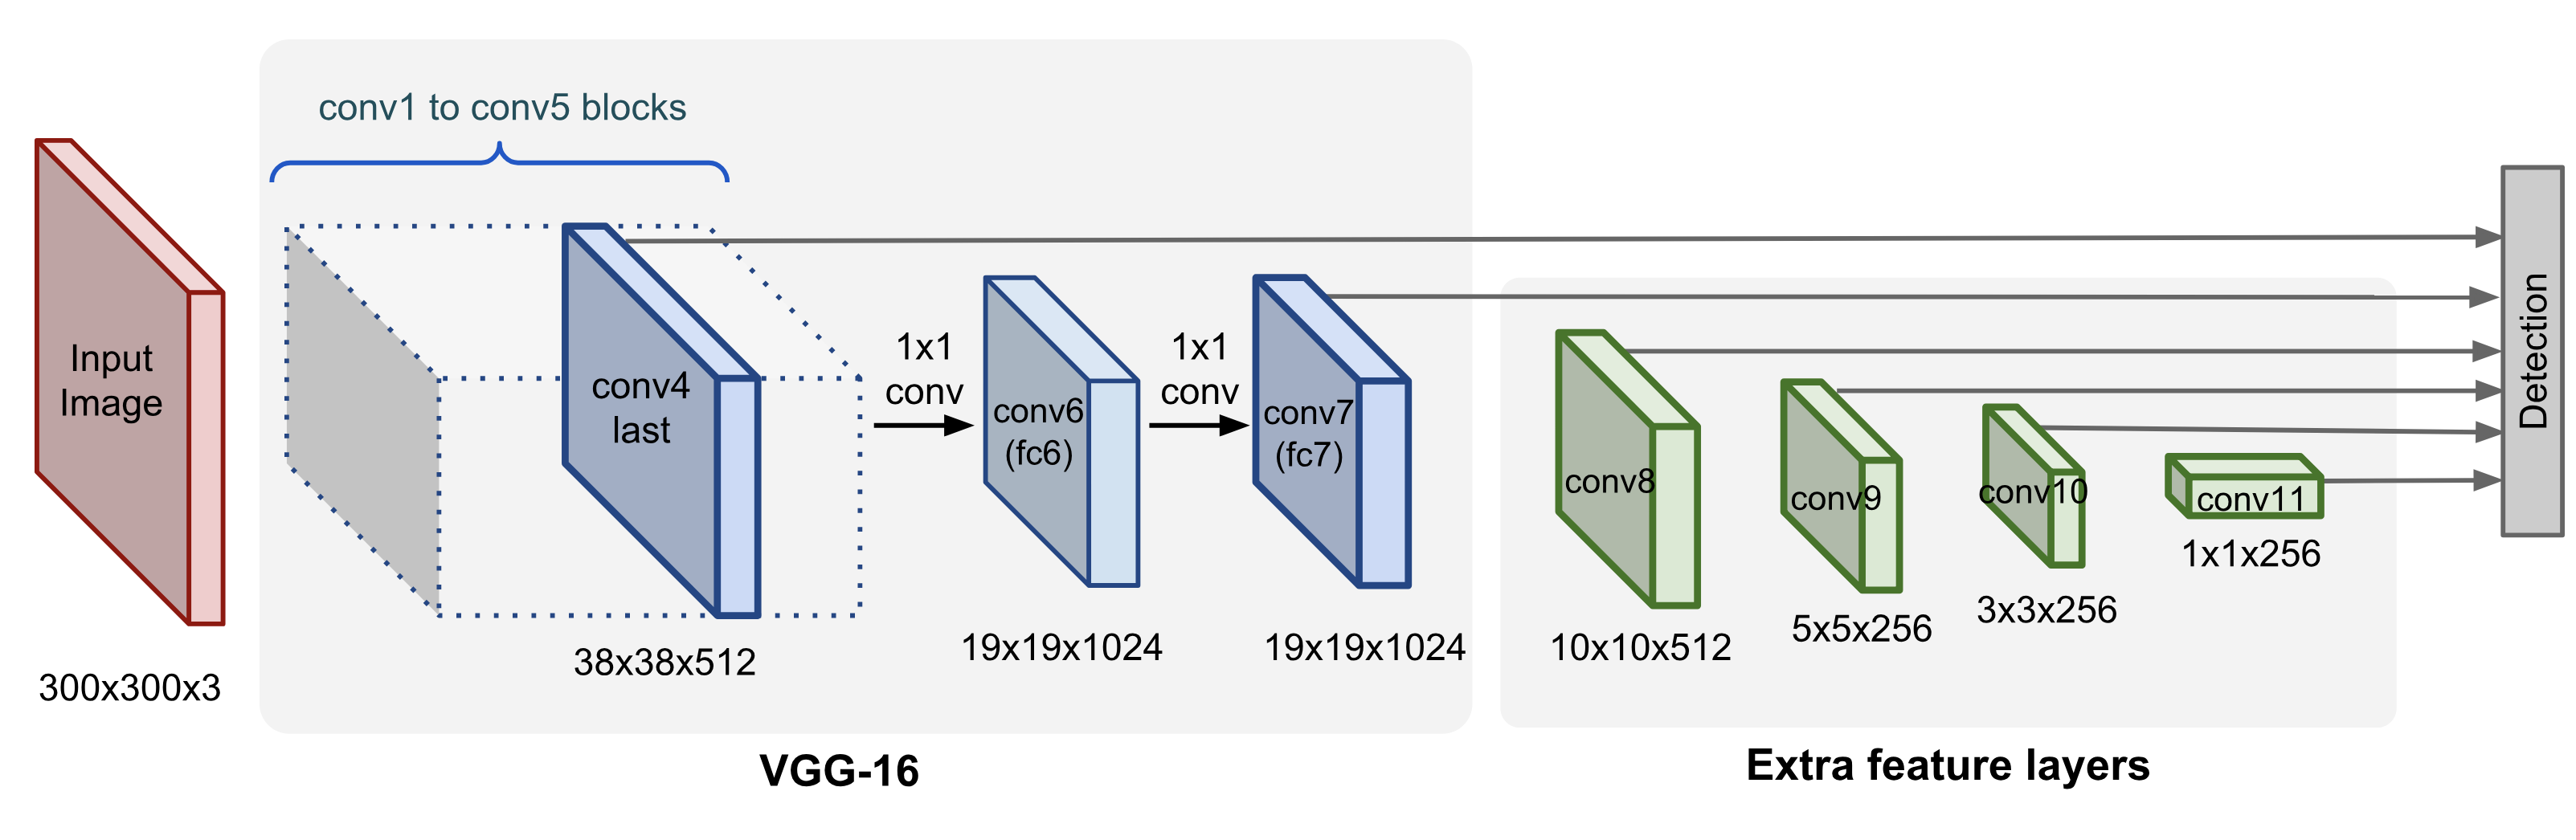
\includegraphics[width=1.0\columnwidth]{.//Figure/Detector/SSD.png}}
 \caption{The SSD architecture. The extra feature layers are responsible for multiple object size detection. Source: \cite{ObjDetArchitectures4}}
 \label{fig:SSD}
\end{figure}

\subsubsection{YOLOv2}

In 2016, YOLOv2\cite{YOLOv2} was introduced and brought numerous improvements over the first version. The v2 architecture uses anchor boxes similar to SSD. Thus, fully connected layers are eliminated. But instead of offsets, YOLOv2 predicts location coordinates relative to the predictor's grid cell location (between 0 and 1). Coordinate (0, 0) is the top left, while (1, 1) is the bottom right of the predictor's cell. This constraint prevents anchor boxes from ending up at any point in the image, stabilizing early training. The default anchor boxes are chosen by running K-Means clustering on the training set. SSD uses various feature maps to get objects of different resolutions. YOLOv2 uses the last convolutional feature map and adds one extra passthrough connection from a previous, higher-resolution layer. The high-resolution features are downscaled by stacking the neighboring features into different channels, turning the spatially bigger feature map to the same size as the last layer, making them concatenable. YOLOv2 also introduced a new CNN backbone, Darknet-19, an ImageNet pre-trained model with batch normalization. It has significantly fewer operations than SSD's VGG-16. During training, the authors used multi-scale training and different augmentations. 

YOLO9000 is a particular v2 variant trained on the COCO (localization+classification) and the ImageNet (classification) datasets with a WordTree model and conditional probability. It can distinguish 9000 different classes thanks to a hierarchical label assignment technique.

\subsubsection{RetinaNet}

RetinaNet\cite{RetinaNet} is an architecture published in 2017 addressing the previously stated negative-positive class imbalance issue. 

This solution uses Smooth L1 loss similarly to SSD for box localization but proposes focal loss for classification. Generally, the class imbalance encountered during training can overwhelm cross-entropy loss. SSD uses hard example mining to resolve this. Focal loss is a dynamically scaled cross-entropy loss. The scaling factor decays to zero as confidence in the correct class increases so that the function can weigh, thus handling class imbalance. The publication uses binary cross-entropy (BCE, also called sigmoid cross-entropy), a sigmoid activation plus a cross-entropy loss. Unlike softmax, BCE is independent for each vector component (class), meaning that the loss computed for every output vector is not affected by others. That is why BCE is used for multi-label classification, where an element belonging to a specific class should not influence the decision for another class. Binary cross-entropy is faster than multi-class cross-entropy, and the name comes from that it sets up a binary classification problem between \(C=2\) types for every class in \(C\). This loss is also helpful to avoid exponential overflow. 

RetinaNet uses the ResNet-50 network as a backbone and takes three different convolutional layer outputs to build a Feature Pyramid Network (FPN). The FPN has a bottom-up path with feature downscaling (the selected ResNet layers are the key levels), then a top-down path with upscaling by the nearest neighbor algorithm. There are lateral connections (element-wise addition) between the corresponding levels of the two pathways. The FPN module generates semantically stronger feature maps on all pyramidal levels, resolving the problem of too low-level features and thus weak earlier layer predictions (responsible for smaller objects). Finally, for each FPN level output, a decoupled classification- and localization head is connected (convolutional layers) to generate outputs for each anchor box level. The high-level structure is shown in Figure \ref{fig:RetinaNet}.

\begin{figure}[htb]
 \centerline{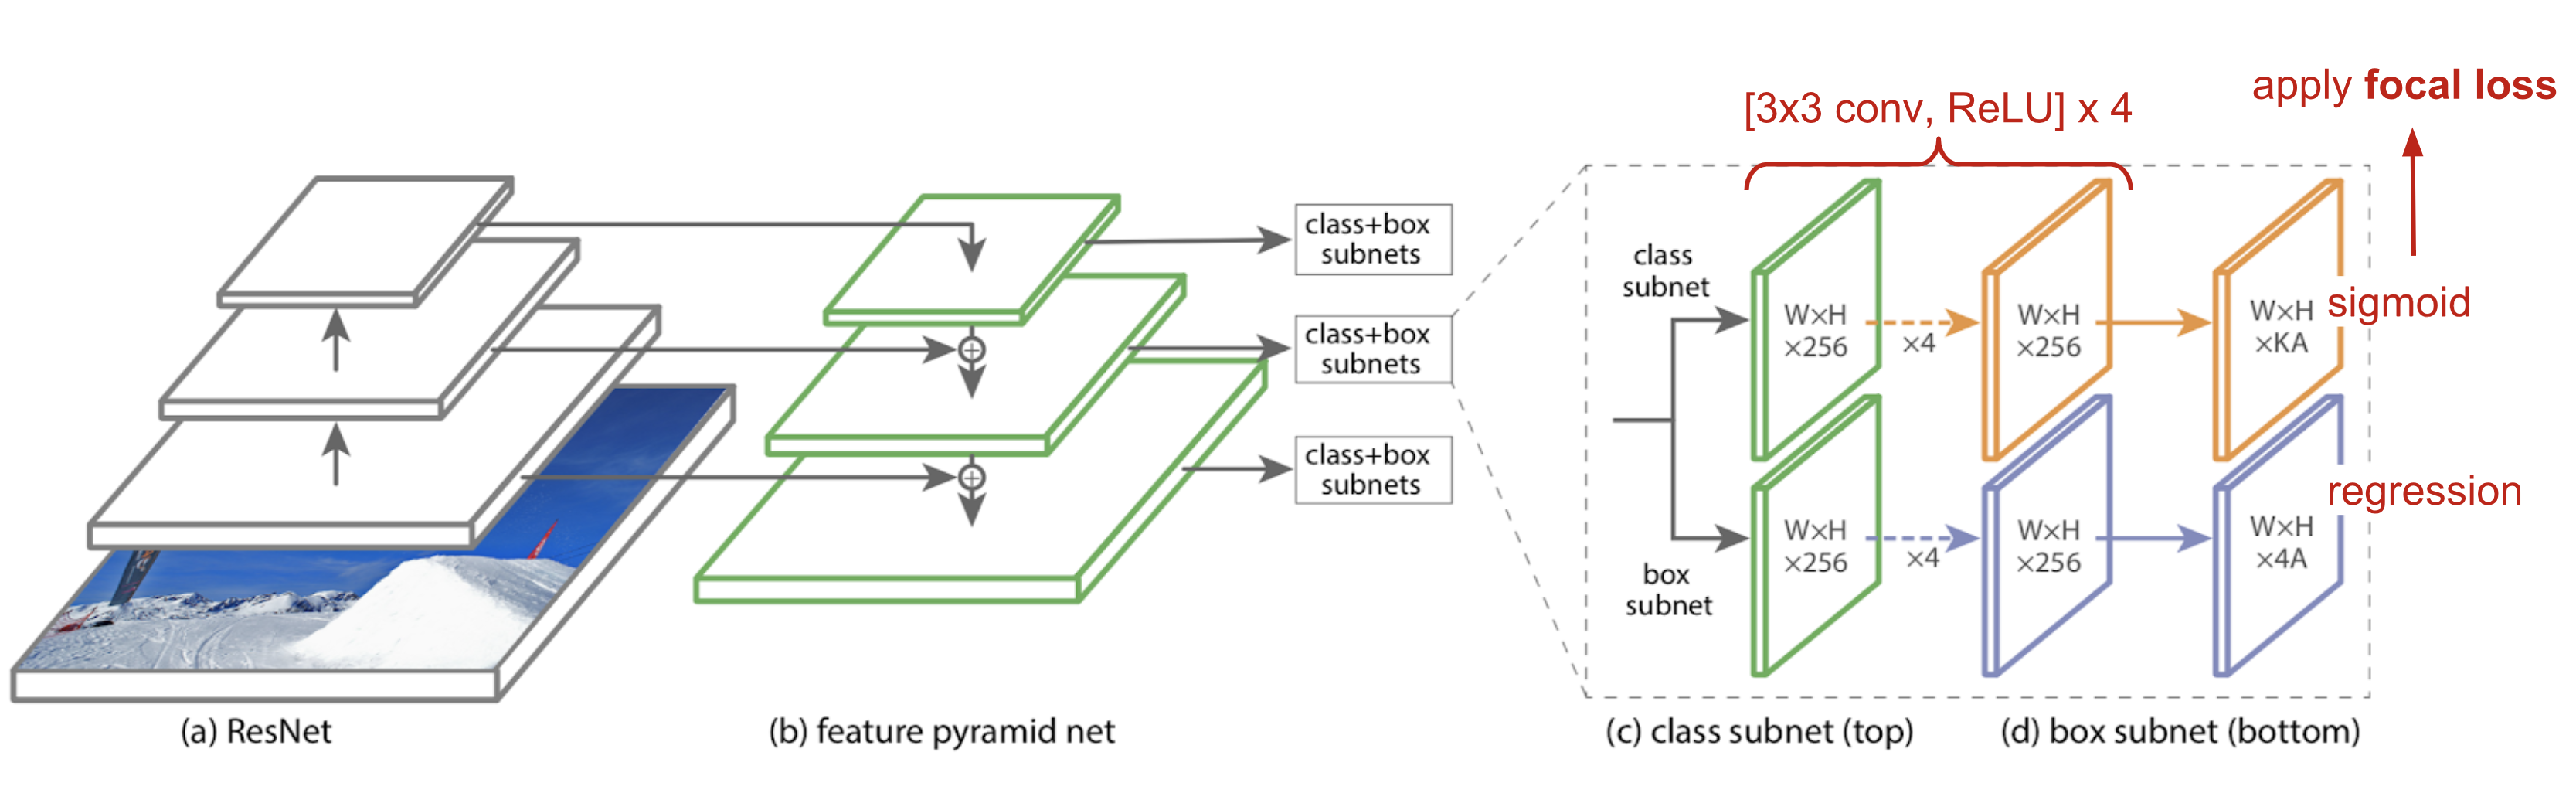
\includegraphics[width=1.0\columnwidth]{.//Figure/Detector/RetinaNet.png}}
 \caption{The RetinaNet architecture. The (a) part is the backbone network whose different level features serve as inputs to the upscaling FPN module (b). A separate predictor head (c-d) is associated with each FPN layer. Source: \cite{ObjDetArchitectures4}}
 \label{fig:RetinaNet}
\end{figure}

RetinaNet uses anchor boxes similarly to SSD, with multiple level anchors. A single predictor outputs cell offsets and anchor rescaling ratios. The architecture introduced novel concepts; it was accurate and robust. However, the deep backbone, the FPN module, and the massive amount of multi-level anchor boxes result in slower running times.

\subsubsection{YOLOv3}

YOLOv3\cite{YOLOv3} was published in 2018, presenting incremental improvements over YOLOv2. In this version, the softmax activation for class prediction is replaced by binary cross-entropy, making class prediction values for an object independent from each other. Also, the objectness score is predicted by logistic regression (binary cross-entropy) instead of the sum of squared errors in the previous YOLOs. Focal loss is not used as the YOLO variants already output objectness scores and downscale losses based on them.

YOLOv3 incorporates the idea of FPN to make predictions at three different scales similar to RetinaNet. The backbone has been replaced with a new model named DarkNet-53, similar to ResNet (deeper network with skip connections).

\begin{figure}[htb]
 \centerline{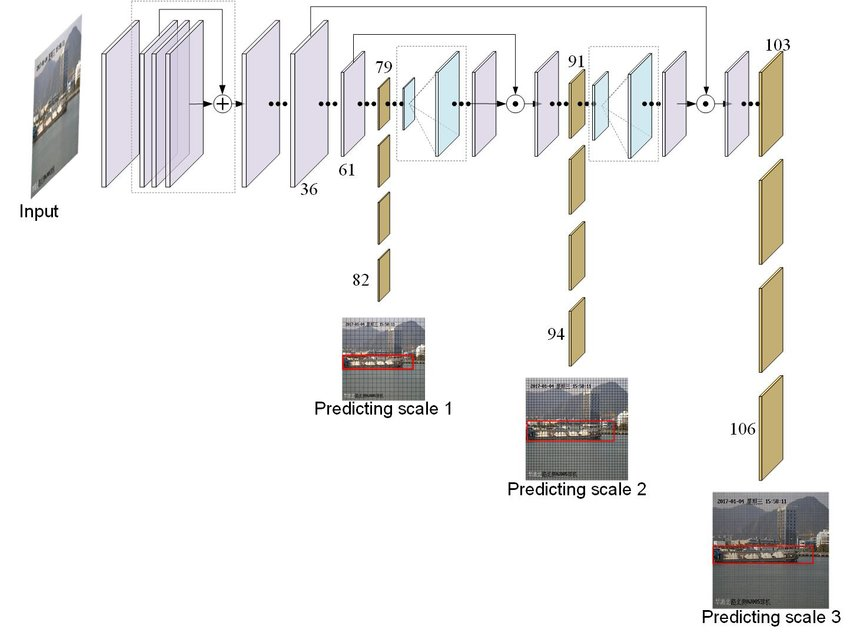
\includegraphics[width=0.8\columnwidth]{.//Figure/Detector/YOLOv3.png}}
 \caption{The YOLOv3 architecture is similar to RetinaNet. For each scale, a coupled predictor head provides the detector outputs. Source: \cite{DeepLearningShipDetection}}
 \label{fig:YOLOv3}
\end{figure}

YOLOv3 compromises speed and accuracy: the deeper backbone and the FPN make it slower than its predecessor. Still, it is more than three times faster than the original RetinaNet and just slightly less accurate, which made YOLOv3 a de-facto industrial solution for years.

\subsubsection{EfficientDet}

EfficientDet\cite{EfficientDet} was introduced in July 2020 by Google Brain and was the benchmark on the COCO dataset in 2020 (55.1 mAP). It is an anchor-based architecture family of object detectors. The paper has proposed the bidirectional Feature Pyramid Network (biFPN), which learns to weigh input features with different resolutions before fusing them. EfficientDet uses EfficientNet CNN backbones, which were engineered with the help of Neural Architecture Search (an automatic process of designing neural networks). The EfficientDet architecture is similar to RetinaNet. It is illustrated in Figure \ref{fig:EfficientDet}.

\begin{figure}[H]
 \centerline{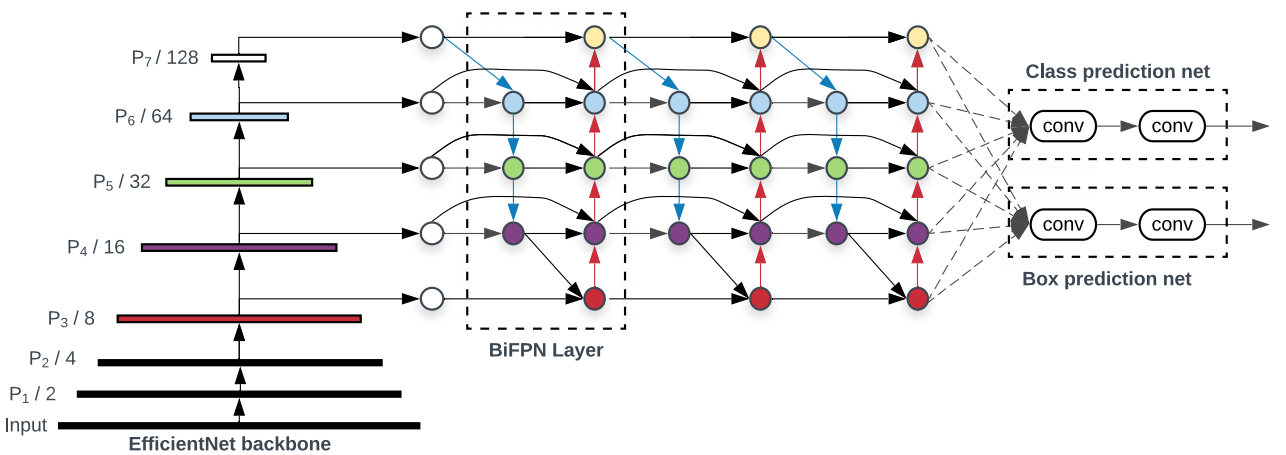
\includegraphics[width=1.0\columnwidth]{.//Figure/Detector/EfficientDet.png}}
 \caption{The EfficientDet architecture learns to weigh features from different FPN levels. Source: \cite{EfficientDet}}
 \label{fig:EfficientDet}
\end{figure}

Over time, a massive number of new solutions emerged. The state-of-the-art solutions on the COCO dataset (as of December 2021) use transformer-based neural networks (like SwinV2-G(HTC++) or Florence CoSwin-H), different from the CNN-based approaches. These are computationally heavy algorithms, making them unsuitable for real-time inference.

The fast-running YOLOv4\cite{YOLOv4} introduced further data augmentation and regularization techniques, a smaller backbone, and the Mish activation function. A month after YOLOv4, YOLOv5\cite{YOLOv5} was released. These architectures, however, do not contain significant modifications. Personally, it feels like they are a bit overly optimized to the anchor-based pipeline. For this reason, I do not discuss them. Instead, I touch anchor-free detectors in the following part, which has been the subject of numerous publications in recent years.

\subsubsection{CenterNet}

CenterNet\cite{CenterNet} was released in 2019, and it uses a different approach compared to other architectures presented so far. It is based on the keypoint-based CornerNet backbone and uses triplets to localize objects. It first generates two coordinates \((XY\textsubscript{min}, XY\textsubscript{max})\) localizing a proposal, then takes its geometric center as the third point. Then, it inspects whether the center key point's region is predicted as the same class as the whole bounding box. This way, the box borders and its central region's visual patterns are analyzed, providing a more robust approach to reduce false positives. CenterNet does not use anchor boxes.

\begin{figure}[htb]
 \centerline{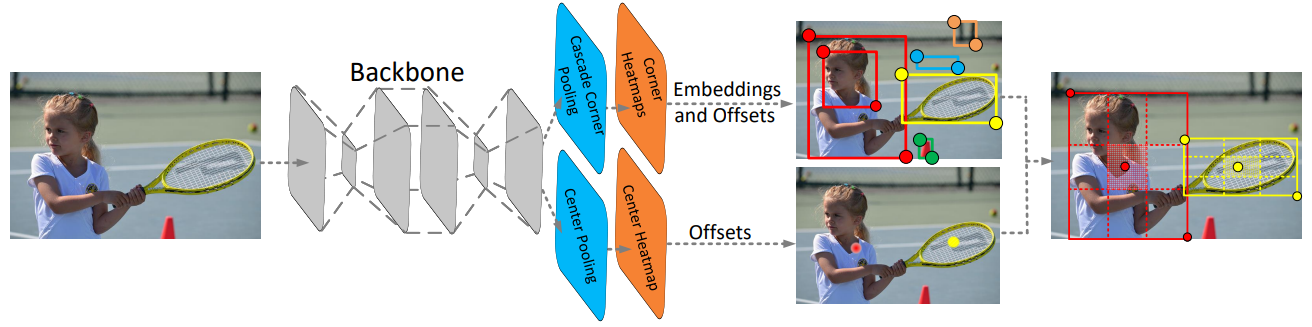
\includegraphics[width=1.0\columnwidth]{.//Figure/Detector/CenterNet.png}}
 \caption{The CenterNet architecture. Source: \cite{CenterNet}}
 \label{fig:CenterNet}
\end{figure}

\subsubsection{YOLOX}

YOLOX\cite{YOLOX} is a publication from August 2021 presenting an anchor-free version of YOLOv3. The authors chose v3 as the starting point because it is widely used, while later variants are overly-optimized, and insufficient software support cannot leverage their capabilities. This architecture slightly modifies v3's loss function, using Complete IoU loss\cite{IoULosses} for the regression (localization) branch. For both the classification- and objectness branches, it uses binary cross-entropy.

YOLOX replaces the coupled detection head with decoupled heads, one each for classification and for localization per feature-pyramid level. The head structure can be seen in Figure \ref{fig:YOLOX_decoupled_head}. Anchor mechanism increases detection head complexity, and the massive number of predictions for each image makes it a bottleneck. YOLOX does not use anchor boxes. Instead, each grid location predicts a single bounding box by four offsets: \(Xmin, Ymin, width, height\). While training, each ground truth box's center location is assigned to the grid cell where it falls in as the positive sample. For each FPN level, a different scale range is predefined in which the current level grid cell can offset its prediction. Center sampling is also used in YOLOX, assigning the central portion cells of ground-truth boxes as positive samples. The label assignment strategy applied is called SimOTA. It first calculates the pairwise matching value for each prediction-ground truth pair by the loss function. Then it selects the top k predictions within the center region as positive samples, while the others are negatives.

\begin{figure}[htb]
 \centerline{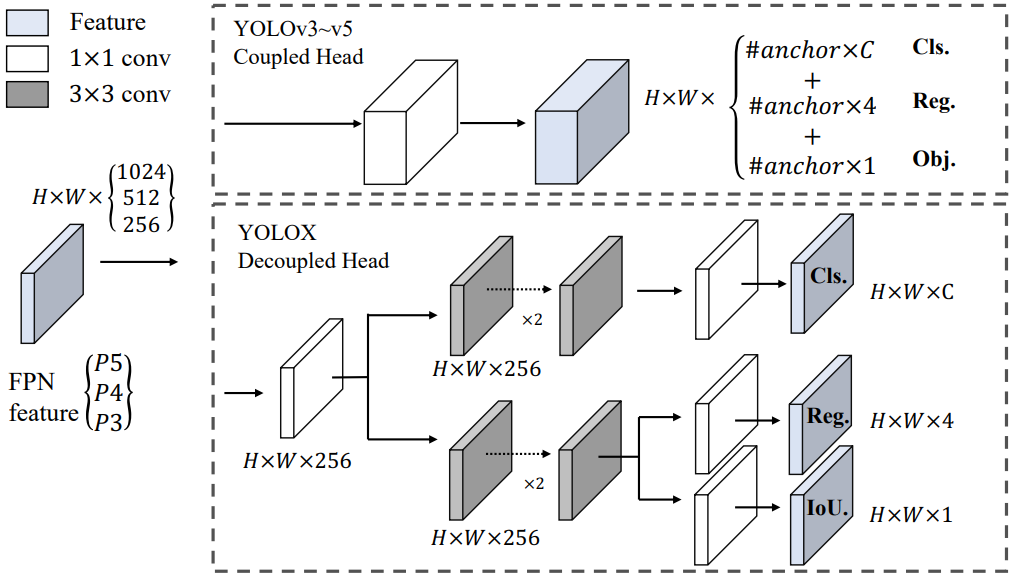
\includegraphics[width=1.0\columnwidth]{.//Figure/Detector/YOLOX_decoupled_head.png}}
 \caption{Decoupled head of YOLOX, which slightly increases runtime but improves accuracy by delegating classification and regression to different branches. Source: \cite{YOLOX}}
 \label{fig:YOLOX_decoupled_head}
\end{figure}

In this part, I presented a few key object detector solutions. The list is not exhaustive, as I didn't describe many other architectures, like EfficientDet, FCOS, NanoDet, and the current state-of-the-art Transformer detectors. The aim of this section was to give an illustration of the basic ideas behind real-time object detection systems.